
\label{chap:results}

The main results of this thesis are grouped into three different sections according to the main phenomena of interest and the used methods. Sections \ref{sec:results_anharm} and \ref{sec:results_interference} summarize the results of non-equilibrium molecular dynamics (NEMD) modeling of lattice heat transfer in various geometries, focusing on anharmonic scattering and wave interference phenomena, respectively. Section \ref{sec:results_gf} highlights the Green's function approach to modeling (i) quantum effects in phonon transport and (ii) cavity-enhancement of electromagnetic energy transfer.


\section{Anharmonic effects in phononic thermal conduction}
\label{sec:results_anharm}

Phonon-phonon scattering arises from the anharmonic terms in the interatomic potential as discussed in Sec. \ref{sec:th_eom2}. These terms are crucial in first-principles modeling of thermal conduction at interfaces and bulk, because they (i) assist heat transfer across interfaces \cite{} and (ii) are responsible for bulk thermal resistivity in pristine materials. Combining molecular dynamics method accounting for anharmonic terms at all orders and the spectral decomposition formula for the heat current [Eq. \eqref{eq:th_spectral_curr}], one can obtain a detailed picture of the effect of these non-linear terms on thermal conduction. Subsection \ref{sec:results_interface} studies the heat current spectrum at the interface between two mass-mismatched materials at different temperatures, revealing two different heat transfer mechanisms relying on anharmonic effects. Subsection \ref{sec:results_mfps} reviews the results for spectral heat current in carbon nanotubes, allowing for determining phonon mean free paths at each vibrational frequency. 

Finally, non-equilibrium molecular dynamics is used in Subsection \ref{sec:results_twinning} to investigate the effects of twinning on the thermal conductivity in silicon nanowires. The results suggest that twinning could be used to increase the thermoelectric figure of merit in silicon nanowires. 

\subsection{Interfacial thermal conduction}
\label{sec:results_interface}

The role of anharmonic phonon scattering in interfacial thermal conduction was investigated using the computational setup presented earlier in Fig. \ref{fig:th_spectral_geom}. Atoms with masses $m_{\textrm{Ar}}=28$ amu and $4m_{\textrm{Ar}}$ were placed in a face-centered cubic lattice, with the atoms of different masses being located in the left and right half-spaces as depicted in Fig. \ref{fig:th_spectral_geom}. The mass-mismatch induces an acoustic mismatch between the materials, inducing a non-zero contact resistance for phonons. Interatomic interactions were modeled using the Lennard-Jones potential \cite{allentildesley} and the parameters were chosen to correspond to solid argon \cite{allentildesley}. More simulation details are found in \citepub{spectral}. % To model acoustic mismatch between the materials, the atomic mass at one side of the interface was chosen to be four times the mass of solid argon, which was the atomic mass on the other side. 

\begin{figure}[tb]
 \begin{center}
  %\includegraphics[width=.99\columnwidth]{/Users/saaskilak/Documents/matlab/pics/171213a_cnt.ps}
 % \includegraphics[width=.99\columnwidth]{/Users/saaskilak/Documents/latex/pics/240114_fcc_final.ps}
  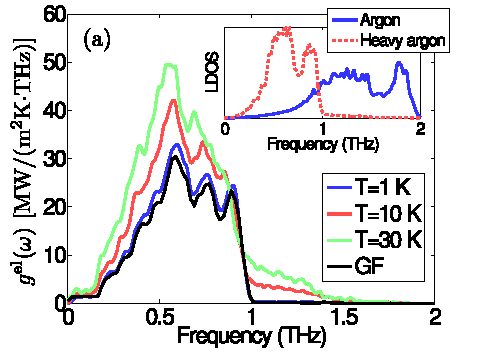
\includegraphics[width=.49\columnwidth]{pics/nemd_fig4a.pdf}
  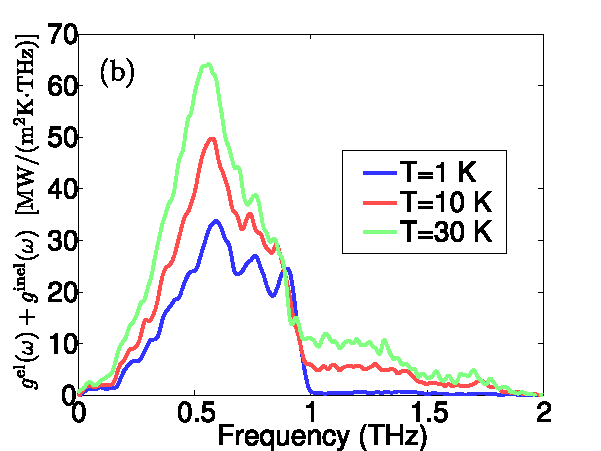
\includegraphics[width=.49\columnwidth]{pics/nemd_fig4b.pdf}
  \caption{Elastic thermal conductance $g^{\textrm{el}}(\omega)=q(\omega)/\Delta T_b$ through the acoustically mismatched interface as a function of frequency at various temperatures.  At $T=1$ K, the elastic conductance agrees with the Landauer-B\"uttiker conductance calculated using the Green's function (GF) method. At high temperatures, anharmonic scattering in the bulk enables energy transfer even above the cut-off frequency of the heavier solid, located at 1 THz.  Inset: Local density of vibrational states (LDOS, arbitrary units) at the interface. Although phonons cannot propagate in the heavier bulk above 1 THz, there are evanescent wave states extending up to 1.5 THz at the vicinity of the interface. (b) The sum $g^{\textrm{el}}(\omega)+ g^{\textrm{inel}}(\omega)$ of elastic and inelastic spectral conductance as a function of frequency. The inelastic conductance describes energy transfer by phonon-phonon interactions across the interface and is defined in detail in \citepub{spectral}. At high temperatures, the anharmonic energy transfer processes strongly enhance interfacial heat transfer at $f\approx 0.5$ THz and above the cut-off of the heavier material (1 THz). Figure reprinted with publisher's permission from \citepub{spectral}.} 
 \label{fig:nemd_fig2}
 \end{center}
\end{figure}

%Interfacial heat transfer mechanisms were investigated by calculating the spectral heat current \eqref{eq:th_spectral_curr} summed over all atomic pairs interacting across the planar interface. By varying the mean temperature $T$, one can investigate the role of anharmonic effects. 

Figure \ref{fig:nemd_fig2}(a) shows the elastic spectral conductance $g^{\textrm{el}}(\omega)=q(\omega)/\Delta T_b$, defined as the spectral current $q(\omega)$ calculated at the interface divided by the temperature jump $\Delta T_b$. Conductance $g^{\textrm{el}}(\omega)$ is referred to as elastic, because it only includes the contributions to interfacial energy transfer by \textit{energy-conserving processes at the interface}, as discussed in detail in \citepub{spectral}. Elastic conductance accounts, however, for the contributions of inelastic effects occurring \textit{in the bulk}. 

As seen in Fig. \ref{fig:nemd_fig2}(a), modes with frequencies above 1 THz cannot carry energy across the interface at low temperature ($T=1$ K), because there are no propagating modes in the heavier material above 1 THz. This absence of modes is evident in the interfacial density of states depicted in the inset of Fig. \ref{fig:nemd_fig2}(a), where only a small tail induced by the evanescent modes is visible above 1 THz in the heavy material. At higher temperatures ($T=10$ K and $T=30$ K), the onset of anharmonic effects can be seen to assist energy transfer across the interface. Most notably, anharmonic effects enable energy transfer even above the cut-off frequency of the heavier material. These high-frequency modes are evanescent in the heavier material, but they can dissipate their heat to lower-frequency modes in the immediate vicinity of the interface through anharmonic interactions. Our results are the first to explicitly demonstrate energy transfer across interfaces by such evanescent wave dissipation.

To further probe the role anharmonic scattering in interfacial energy transfer, we determined also the first-order inelastic contribution to the spectral heat current at the interface. The expression for this inelastic conductance $g^{\textrm{inel}}(\omega)$, corresponding to three-phonon processes at the interface, was derived from the second-order contribution to spectral heat current as detailed in \citepub{spectral}. The sum of elastic and inelastic contributions to the conductance is shown in Fig. \ref{fig:nemd_fig2}(b). Comparison to Fig. \ref{fig:nemd_fig2}(a) shows that the three-phonon energy transfer processes enhance energy transfer across the whole frequency range between zero and 2 THz, both below and above the cut-off frequency of the heavy argon. As discussed in detail in \citepub{spectral}, these three-phonon energy tranfer processes are dominated by frequency-doubling and frequency-halving anharmonic processes at the interface, in support of the phenomenological higher harmonic inelastic model (HHIM) suggested earlier by Hopkins \cite{hopkins09_jap}. Our results are the first to quantify the contributions of such processes from atomistic simulations. Due to the high computational effort required for determining the contributions of even higher-order processes to conductance, the analysis of \citepub{spectral} was limited to first-order anharmonic processes.

\subsection{Mean free paths in carbon nanotubes}

\label{sec:results_mfps}

\begin{figure}[tb]
 \begin{center}
  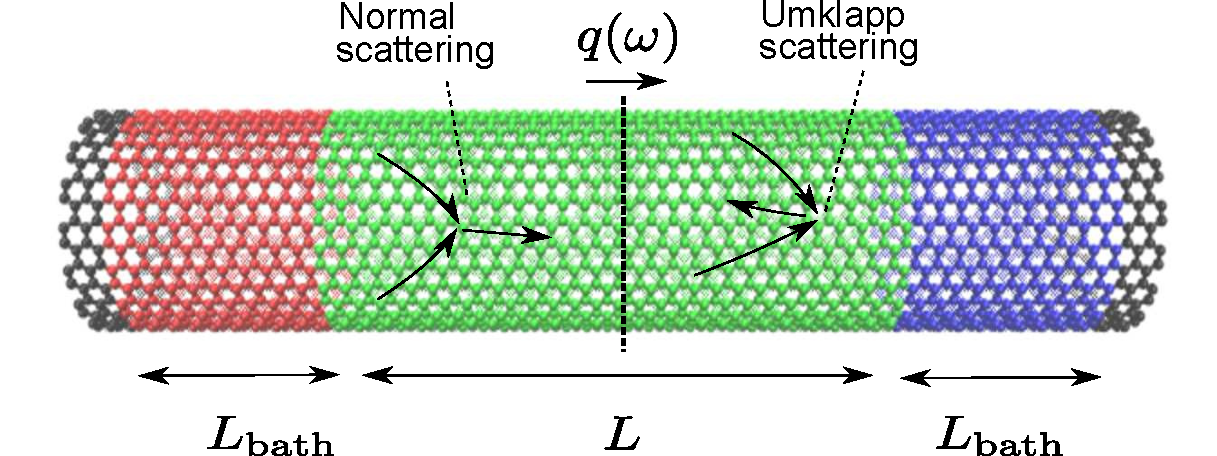
\includegraphics[width=.89\columnwidth]{pics/cnt_fig1-crop.pdf} 
  \caption{Schematic illustration of the NEMD setup used for determining the length-dependent thermal conductivity and phonon mean free paths in carbon nanotubes. When traversing the tube, phonons undergo both normal and Umklapp processes leading to the length-dependence of the spectral heat current $q(\omega)$ in the tube. From the $L$-dependence of $q(\omega)$, one can determine the mean free paths at each frequency as described in \citepub{cnt}. Figure reprinted with publisher's permission from \citepub{cnt}.}  
\label{fig:cnt_fig1}
 \end{center}
\end{figure}

Carbon nanotubes have a very high thermal conductivity in the range 500-5000 W/mK \cite{}, and their thermal conductivity has been found to increase as a function of tube length in tubes as long as 5 $\upmu$m and, very recently, in tubes as long as 1 mm (C.W. Chang, private communication). The goal of \citepub{cnt} was to shed light to the increase of thermal conductivity in pristine nanotubes by determining the frequency-dependent phonon mean free paths from atomistic simulations by investigating the length-dependence of spectral heat current \eqref{eq:th_spectral_curr}. % The simulated tube lengths exceed 

Figure \ref{fig:cnt_fig1} shows the schematic illustration of the nonequilibrium molecular dynamics setup used for carbon nanotubes of (10,10) chirality. Regions of length $L_{\textrm{bath}}=10$ nm were coupled to Langevin thermostats at temperatures $T+\Delta T/2$ and $T-\Delta T/2$ to drive heat current through the tube, and the frequency-dependent phonon mean free paths were determined from the decrease of the non-equilibrium spectral heat current \eqref{eq:th_spectral_curr} at different frequencies as a function of tube length $L$. The decrease in spectral current arises from anharmonic interactions, which are fully accounted for by the non-linear terms of the optimized Tersoff potential used for modeling carbon-carbon interactions \cite{tersoff88a,lindsay10}. In contrast to equilibrium mean free paths, which characterize the scattering lengths arising from the combined effect of normal and Umklapp processes \cite{mcgaughey04}, the mean free paths determined from NEMD directly reflect the \textit{resistance to the heat flow} (dominated by Umklapp processes). For a detailed account of the method, see \citepub{cnt}.


\begin{figure}[tb]
 \begin{center}
  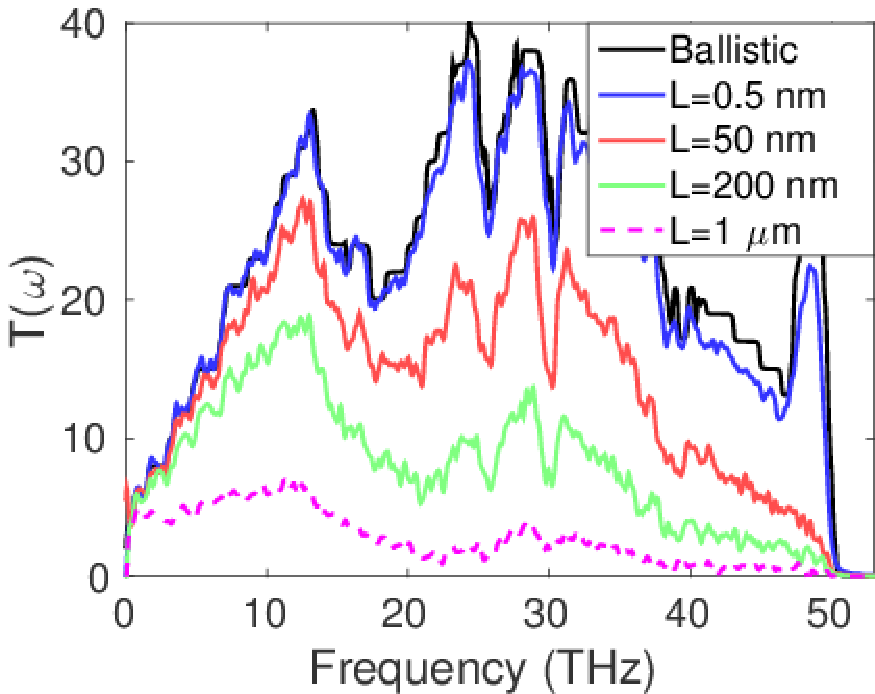
\includegraphics[width=.49\columnwidth]{pics/cnt_fig2.pdf} 
  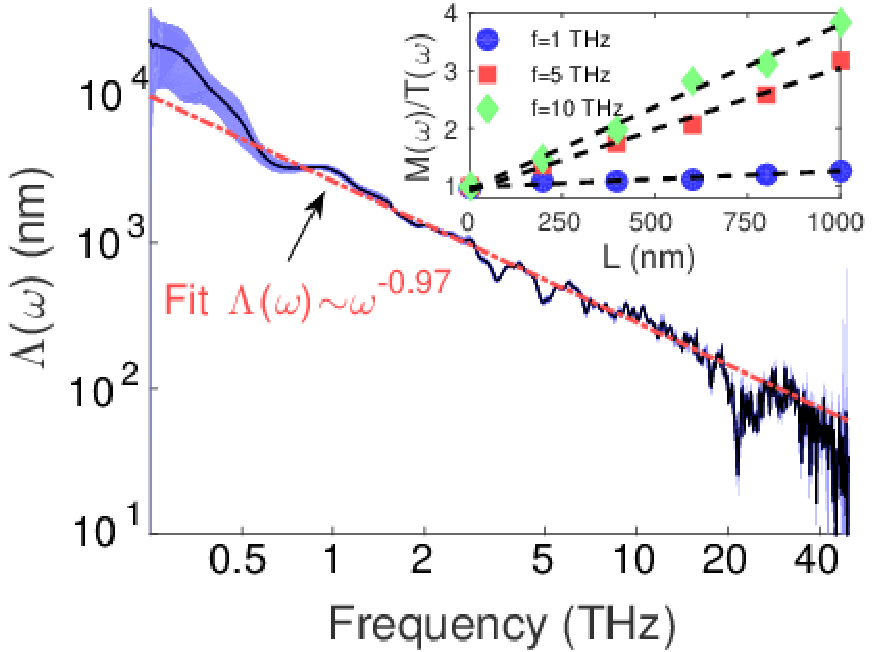
\includegraphics[width=.49\columnwidth]{pics/cnt_fig4.pdf} 
  \caption{(a) Generalized phonon transmission function $\ca{T}(\omega)=q(\omega)/(k_B\Delta T)$ for different tube lengths at $T=300$ K. Increasing the tube length reduces the transmission due to anharmonic scattering. For $L=0.5$ nm, phonon transmission is nearly equal to the ballistic value determined by counting the number of propagating modes in the nanotube. (b) Log-log plot of the mean free path $\Lambda(\omega)$ at $T=300$ K, determined from the slope of the inverse transmission function as a function of tube length $L$ as illustrated by the dashed lines in the inset. The shaded regions in the main figure correspond to the 92.5\% confidence interval for the slope. Below 0.25 THz, the confidence interval is large due to numerical uncertainties, preventing the determination of mean free paths at the lowest frequencies. Figure reprinted with publisher's permission from \citepub{cnt}. \textbf{ADD (A) AND (B)}}  
\label{fig:cnt_fig2}
 \end{center}
\end{figure}

Figure \ref{fig:cnt_fig2}(a) shows the generalized phonon transmission function $\ca{T}(\omega)=q(\omega)/(k_B\Delta T)$ for different tube lengths $L$. This dimensionless quantity is essentially the phonon transmission probability through a tube of length $L$, summed over all propagating modes at angular frequency $\omega$. For $L=0.5$ nm, the transmission probability of each mode is unity and the generalized phonon transmission is nearly equal to the number of propagating phonon modes (black solid line). As the tube length increases, anharmonic scattering reduces the transmission. This reduction is strongest at high frequencies, suggesting that the mean free path descreases as a function of frequency, which is reasonable considering the larger phase-space available for phonon-phonon scattering at high frequencies \cite{ziman}.

Phonon mean free paths are plotted as a function of frequency in Fig. \ref{fig:cnt_fig2}. The mean free paths are calculated using the fitting procedure described in the inset of Fig. \ref{fig:cnt_fig2} and in more detail in \citepub{cnt}. The results show that the mean free paths obey a power-law $\Lambda(\omega)\propto \omega^{-\alpha}$ as a function of frequency in a large frequency interval, with a different exponent ($\alpha\approx 0.97$) than the value $\alpha=2$ used earlier \cite{wang06_apl} to phenomenologically describe the ballistic-diffusive transition in CNTs. At low frequencies, the MFPs exceed 1 $\upmu$m, in agreement with the strong length-dependence of the experimentally measured thermal conductivity in nanotubes as long as $5$ $\upmu$m \cite{chang08}.

\textbf{DISCUSSION}

\subsection{Thermal conductivity reduction in twinning nanowires}

\label{sec:results_twinning}

\begin{figure}[tb]
 \begin{center}
  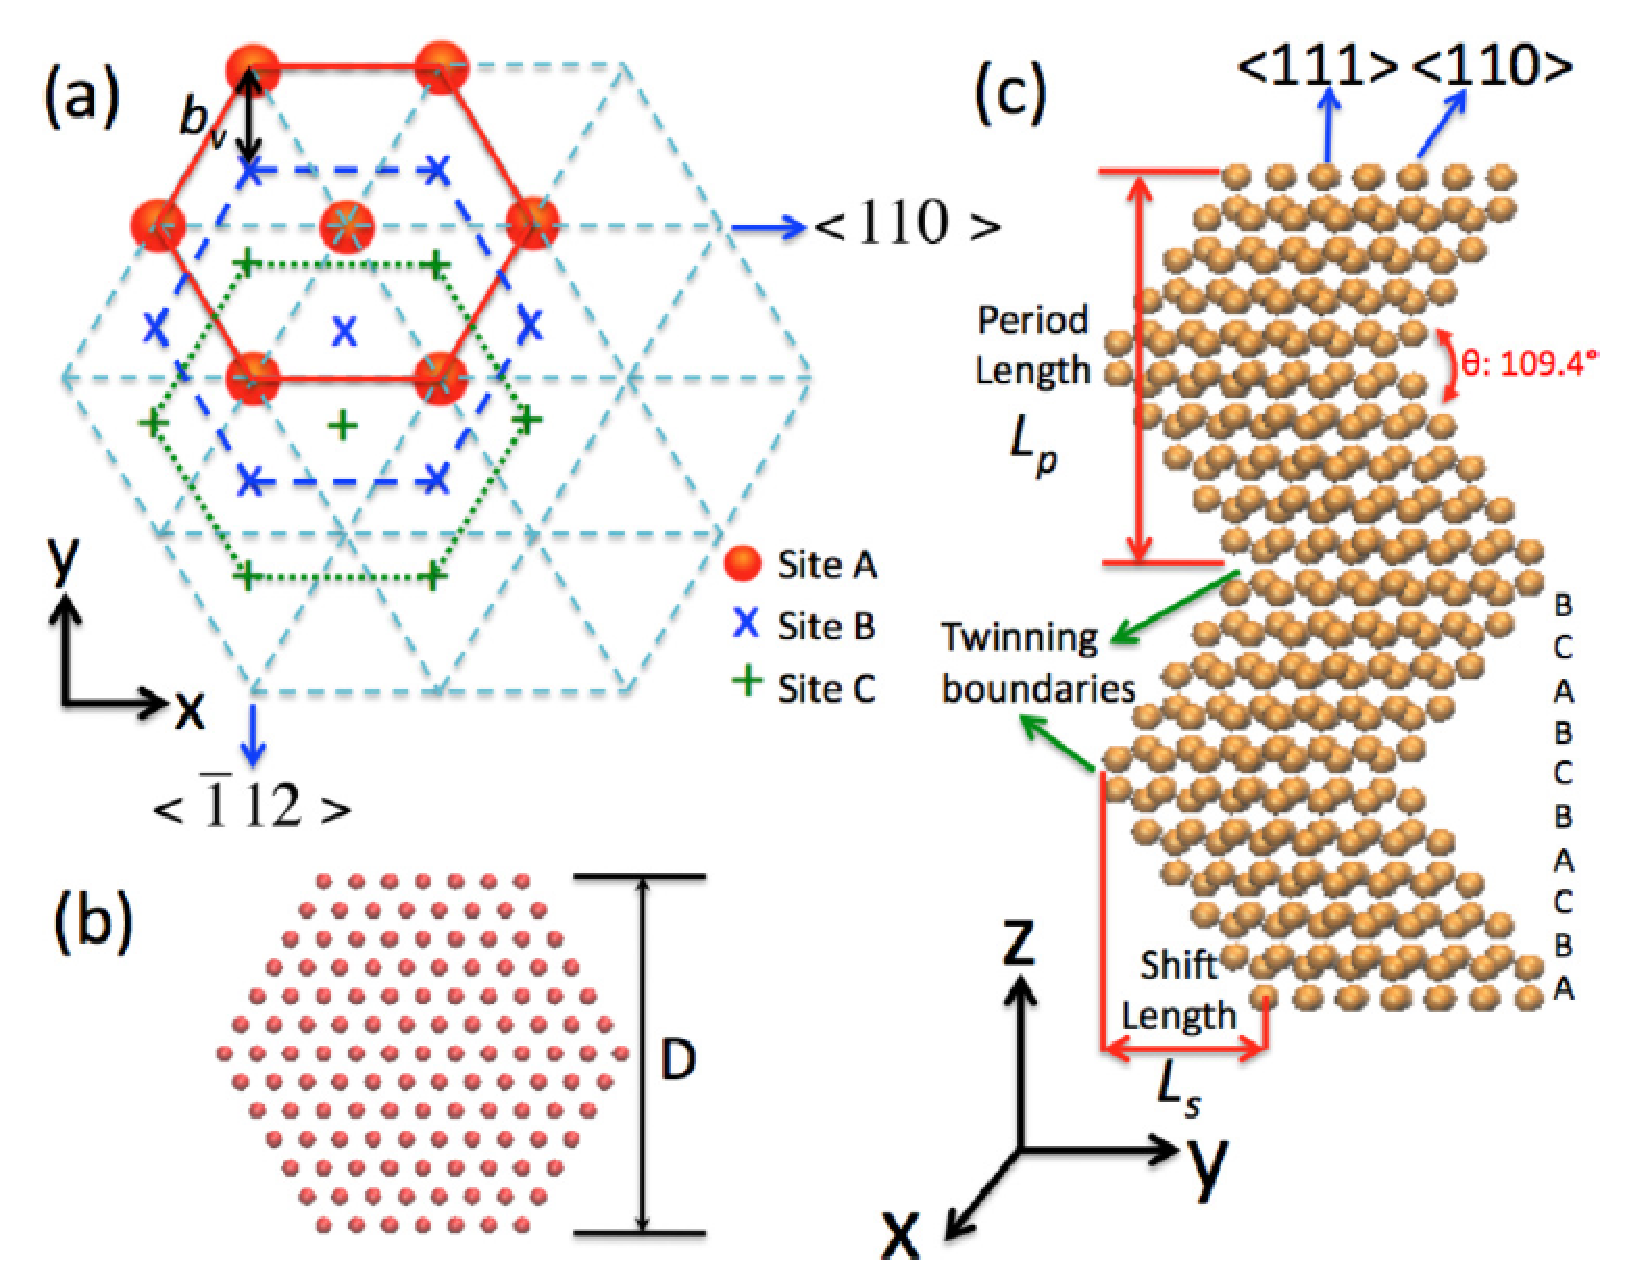
\includegraphics[width=.89\columnwidth]{pics/twinning_fig1.pdf} 
  \caption{(a) Schematic illustration of stacking in the close-packed silicon lattice. Stacking fault occurs when the stacking sequence ABCABC is locally changed to ABCBAC. (b) Cross-section of the nanowire. (c) Silicon nanowire with twinning boundaries. The period length is denoted by $L_p$ and the ''shift length'' $L_s$ is related to $L_p$ by $L_s=(L_p/2)\cot(\theta/2)$, where $\theta=109.4^{\circ}$. The figure also illustrates the perturbation of the ABCABC... stacking sequence at the twinning boundaries. Figure reprinted with publisher's permission from \citepub{twinning}.}  
\label{fig:twinning_fig1}
 \end{center}
\end{figure}

As discussed in Chap. \ref{chap:intro}, solid-state thermoelectric conversion requires materials with low thermal conductivity and high electronic conductivity. To efficiently the reduce thermal conductivity in nanomaterials, anharmonic scattering must be accompanied by other scattering mechanisms such as boundary and impurity scattering. Twinning interfaces are known to reduce thermal conductivity without perturbing electronic transport \cite{}. In \citepub{twinning}, the effect of twinning on the thermal conductivity of Si nanowires was investigated using nonequilibrium molecular dynamics simulations.

% The possibility to tune the geometric parameters presents therefore opportunities for thermal conductivity engineering and, most crucially, reducing thermal conductivity without affecting electron transport. 

% The geometry-induced effect of twinning on the thermal conductivity in silicon nanowires was investigated using NEMD in \citepub{twinning}. In twinning nanowires, phonons are scattered not only by anharmonic scattering (as also in the pristine nanotubes considered in the previous subsection) but also by the twinning-induced zigzag-shaped kinks in the geometry. 

The computational NEMD setup of \citepub{twinning} was similar as for carbon nanotubes, with the exception that Langevin heat baths were replaced by deterministic Nos\'e-Hoover thermostats \cite{nose84} and interatomic potential was replaced by the Stillinger-Weber potential modeling silicon-silicon interactions \cite{stillinger85}. The cross-section of the nanowires was chosen to be hexagonal with diameter $D$ as shown in Fig. \ref{fig:twinning_fig1}(b). The twinning period is denoted by $L_p$, which corresponds to the ''shift length'' $L_s=(L_p/2)\cot(\theta/2)$, where $\theta=109.4^{\circ}$ [see Fig. \ref{fig:twinning_fig1}(c)]. More details are given in \citepub{twinning}.


\begin{figure}[tb]
 \begin{center}
  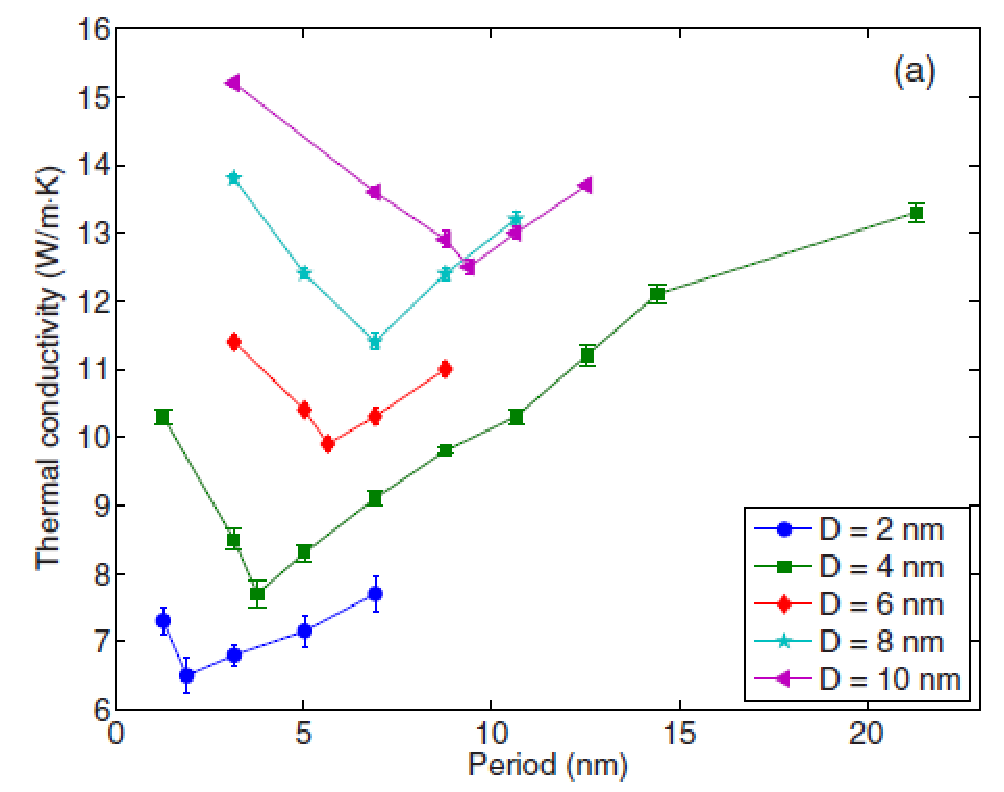
\includegraphics[width=.89\columnwidth]{pics/twinning_fig2a.pdf} 
  \caption{Thermal conductivity of silicon twinning nanowires at $T=300$ K as a function of period length $L_p$ for different diameters $D$. For each diameter $D$, there is a corresponding minimum in the thermal conductivity as a function of period length. The minimum arises from the competition between geometric and anharmonic effects as shown in \citepub{twinning}. Figure reprinted with publisher's permission from \citepub{twinning}. \textbf{REMOVE (A)}}  
\label{fig:twinning_fig2}
 \end{center}
\end{figure}

Thermal conductivity of the twinning nanowires as a function of period $L_p$ are shown in Fig. \ref{fig:twinning_fig2} for different diameters $D$. For each diameter, there is a corresponding period length with a minimum in the thermal conductivity. Lowest conductivity was found for the period length $L_p\approx 0.95D$, corresponding to the shift length $L_s=D/3$. The detailed mechanisms behind the minimum thermal conductivity were analyzed in detail in \citepub{twinning}, with the conclusion that it arises from the competition between geometric and anharmonic scattering. To reduce thermal conductivity even further, this geometric reduction can be used in conjuction with other well-known mechanisms for thermal conductivity reduction such as alloying \cite{}, partial amorphization \cite{}, and coating \cite{}. %  (see \citepub{twinning}). 

While the observed thermal conductivity minimum in twinning nanowires is analogous to the minimum thermal conductivity in superlattices (SLs) \cite{simkin00}, the mechanisms behind the phenomena are different. In SLs, the minimum arises from the interplay between phonon coherence and phonon boundary scattering, with the latter being due to acoustic mismatch at material interfaces. In twinning nanowires, there is no acoustic mismatch at the kinks, so scattering only arises from the geometric effect. Because electron transport is expected to be unhindered by the stacking faults due to the small electron wavelength, the results suggest that the thermoelectric efficiency of twinning nanowires is higher than in their pristine counterparts. % This minimum was found to depend on the shift length as $L_s=D/3$, suggesting that the effect can be explained by geometric scattering. 


\section{Interference effects in phononic thermal conduction through constrictions}
\label{sec:results_interference}

In many applications, it is desirable to electrically and thermally insulate the contact between two bulk materials by a vacuum gap separation \cite{}. It is, however, difficult to support such structures without nanoscale point contacts bridging the gap. Such point contacts conduct heat and can therefore disturb thermal insulation. Thermal conduction properties of point contacts between bulk materials have therefore become of both theoretical \cite{} and experimental \cite{bartsch12} interest in recent years. 

Because the feature sizes of nanoscale point contacts can be comparable to thermal phonon wavelengths, interference effects can play an important role in thermal conduction. Discovery of interference effects in point contacts could possibly be exploited for therman conductivity engineering in the same way as in phononic crystals \cite{maldovan13}. % and nanocapacitors \cite{han15}.

\begin{figure}
\begin{center}
 %\includegraphics[width=8.6cm]{../scbaths_paper_re_resubmission/pic1.ps}
 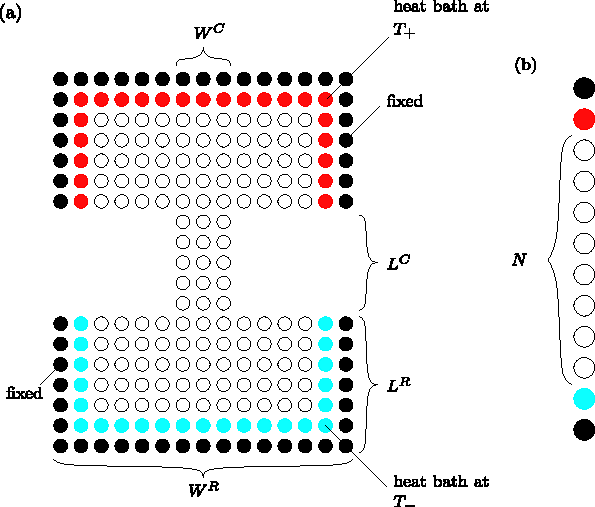
\includegraphics[width=.85\columnwidth]{pics/fpu_fig1.pdf}
 \caption{Schematic illustration of the simulation setup for a point contact in a two-dimensional square lattice. Figure reprinted with publisher's permission from \citepub{fpu}. \textbf{(b) TO BE REMOVED.}}
\label{fig:fpu_fig1}
\end{center}
\end{figure}

To investigate interference effects in point contacts, we performed nonequilibrium molecular dynamics simulations using the simulation setup schematically illustrated in Fig. \ref{fig:fpu_fig1}. Atoms were placed in a square lattice, with the particles at the boundaries of the bulk parts at the top or bottom being either fixed (black circles) or coupled to Langevin baths at temperature $T_+$ (red circles) or $T_-$ (cyan circles). In \citepub{fpu}, the large bulk parts were connected by a rectangular point contact that is $L^C$ atoms long and $W^C$ atoms wide. Triangular and discoidal shaped point contacts were considered in \citepub{fpu2}. 
% Anharmonic phonon-phonon scattering, which is responsible for decoherence and therefore loss of interference, is accounted for by the anharmonic terms in the interatomic potential as discussed below. 

Lattice dynamics in the setup of Fig. \ref{fig:fpu_fig1} was modeled by coupling all nearest-neighbor atom pairs by anharmonic springs (not shown), whose potential energies include both quadratic and quartic terms. This potential was used by Fermi, Pasta and Ulam to investigate thermalization in one-dimensional systems \cite{fermi55} and is therefore called Fermi-Pasta-Ulam potential. The simple form of the Fermi-Pasta-Ulam potential allows for scaling the anharmonicity by a corresponding scaling in temperature, so one can present results for a single value of anharmonicity parameter without loss of generality. This scaling and other simulation details are reviewed in \citepub{fpu}. 


\begin{figure}
\begin{center}
 %\includegraphics[width=8.6cm]{../scbaths_paper_re_resubmission/pic1.ps}
 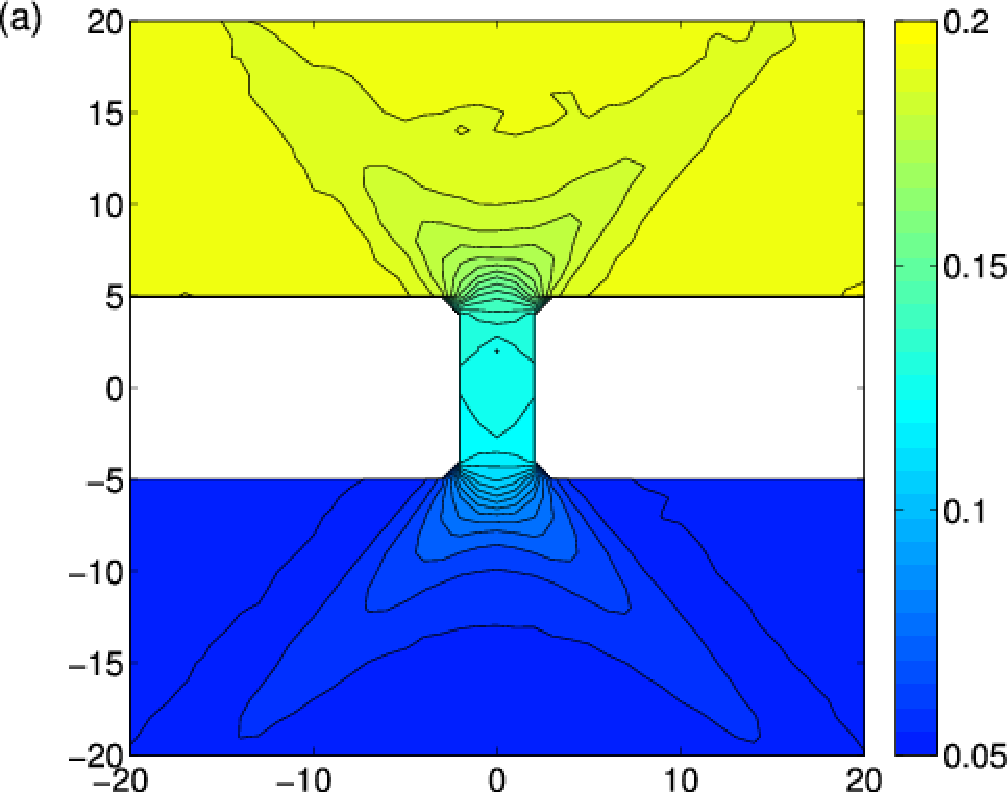
\includegraphics[width=.49\columnwidth]{pics/fpu_fig2a.pdf}
  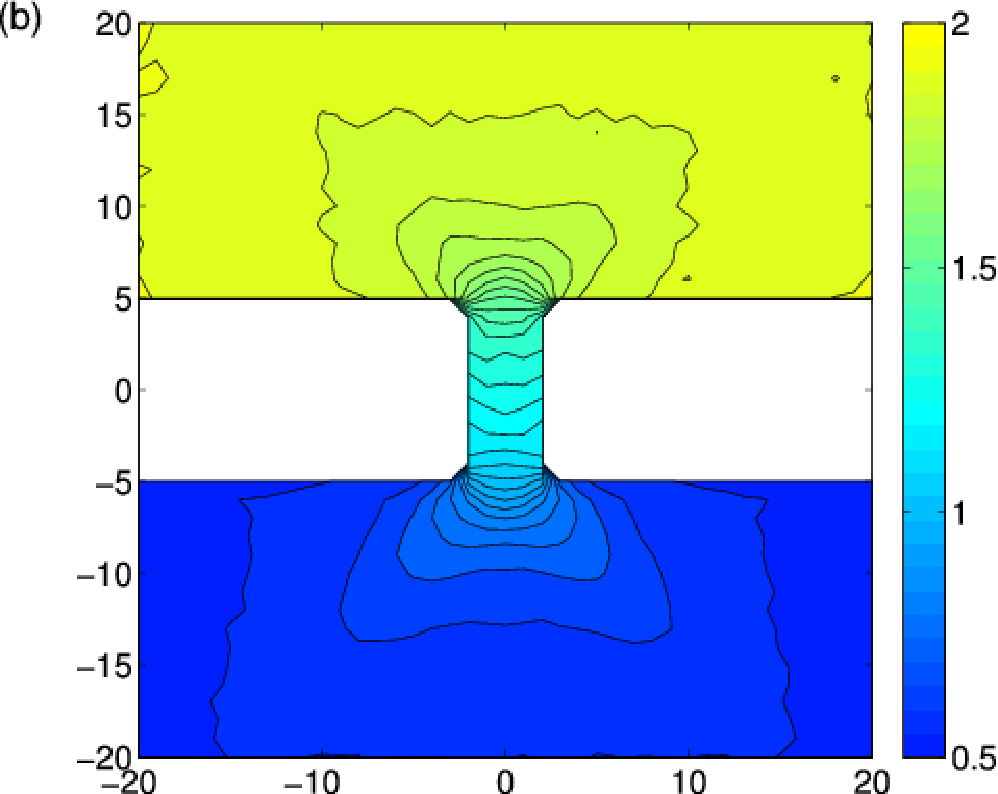
\includegraphics[width=.49\columnwidth]{pics/fpu_fig2b.pdf}
 \caption{Kinetic temperature profile at (a) low temperature ($T_+=0.20$, $T_-=0.05$) and (b) high temperature ($T_+=2.0$, $T_-=0.5$). The bulk size is $W^R=161$, $L^R=80$ and the constriction size $W^C=5$, $L^C=9$ (see Fig. \ref{fig:fpu_fig1}). The labels on the horizontal and vertical axes mark the atom indices. Figure reprinted with publisher's permission from \citepub{fpu}.}
\label{fig:fpu_fig2}
\end{center}
\end{figure}

Figure \ref{fig:fpu_fig2} shows the kinetic temperature $T_i^{\textrm{kin}}=\langle mv_i^2 \rangle/k_B$ at each atomic site $i$ in a contour plot at (a) low temperature and (b) high temperature for a rectangular constriction of length $L^C=9$ and width $W^C=5$. Temperatures are given in dimensionless units defined in \citepub{fpu}. At low temperature, lattice waves can propagate without losses and, therefore, temperature is nearly constant in the constriction. Most notably, the lossless propagation can be seen to induce wavelike-features in the kinetic temperature profile in the bulk parts,with directional features along the $\langle 11 \rangle$ crystal directions. Such features are in contrast with Fourier's law predicting a highly symmetric temperature profile with no directional features (not shown). When temperature is increased [Fig. \ref{fig:fpu_fig2}(b)], the directional features vanish and temperature profile becomes more similar to Fourier's law's prediction. Temperature profile also develops a non-zero gradient inside the constriction due to smaller thermal conductivity.


\begin{figure}
\begin{center}
 %\includegraphics[width=8.6cm]{../scbaths_paper_re_resubmission/pic1.ps}
 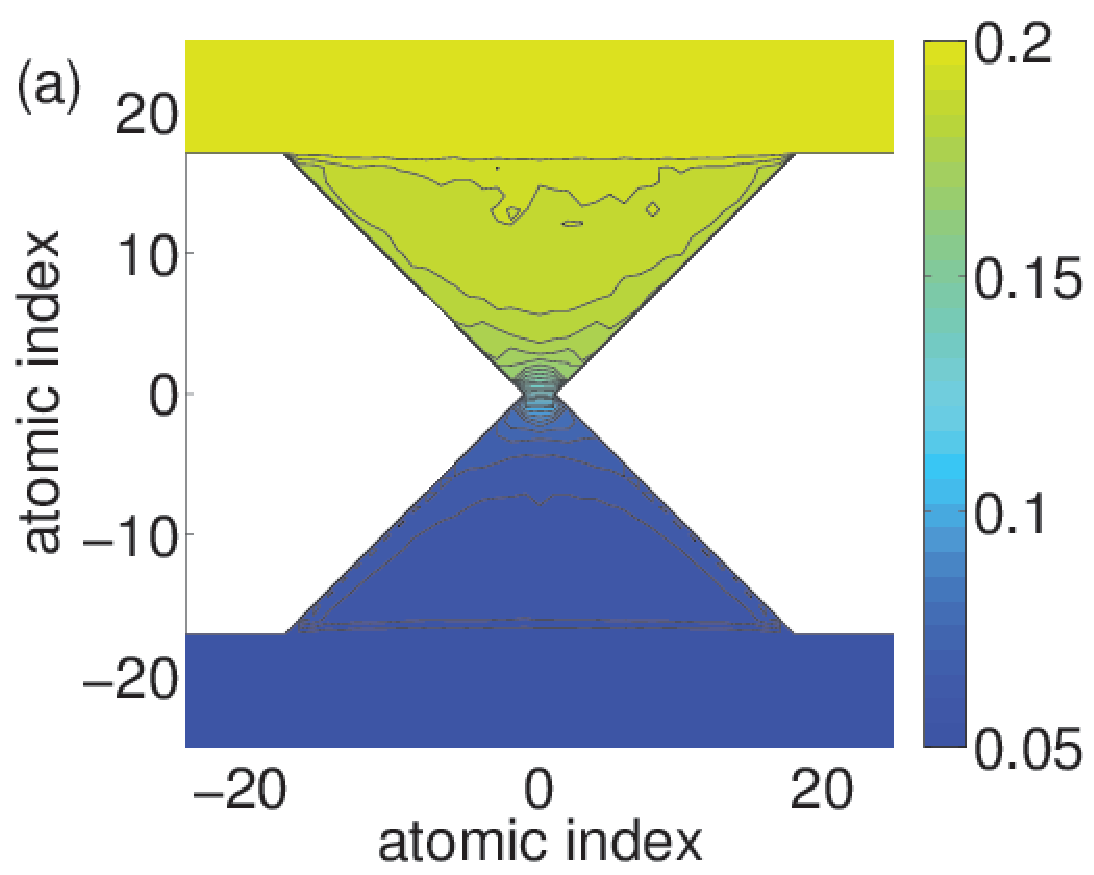
\includegraphics[width=.49\columnwidth]{pics/aip_fig5a.pdf}
 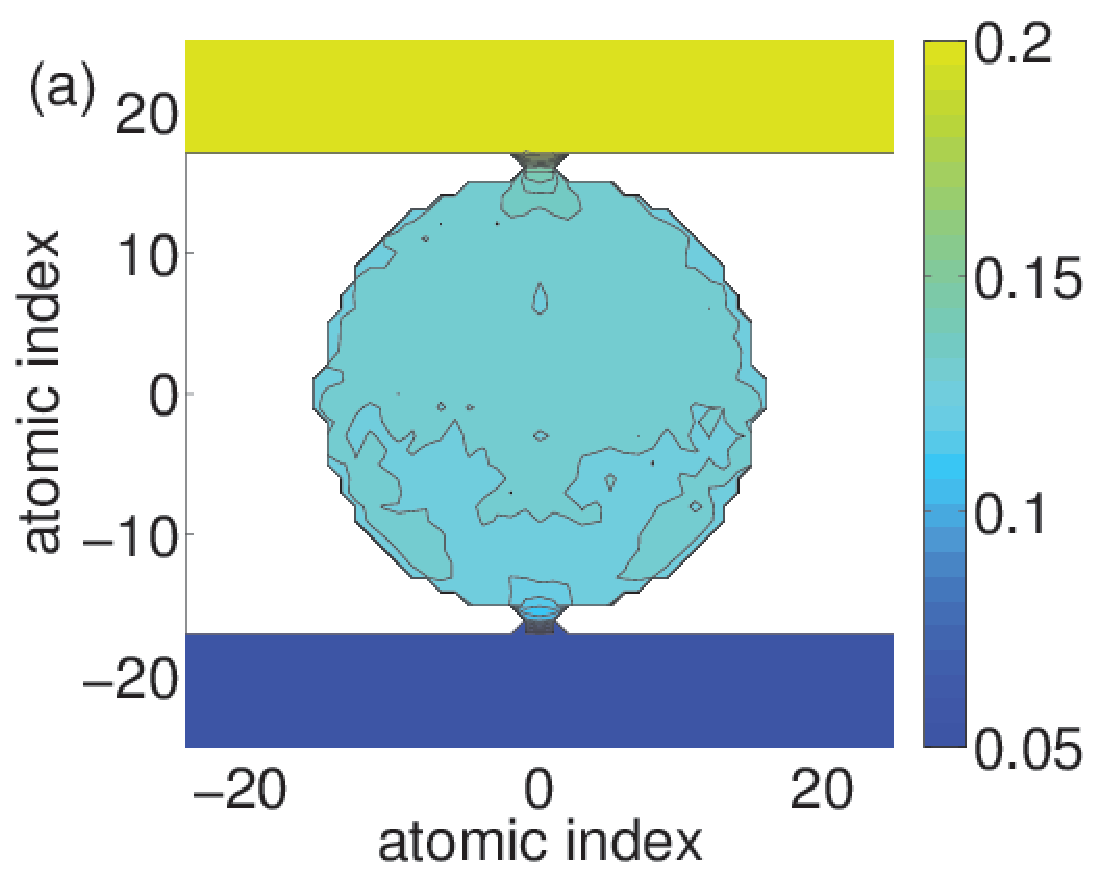
\includegraphics[width=.49\columnwidth]{pics/aip_fig6a.pdf}
 %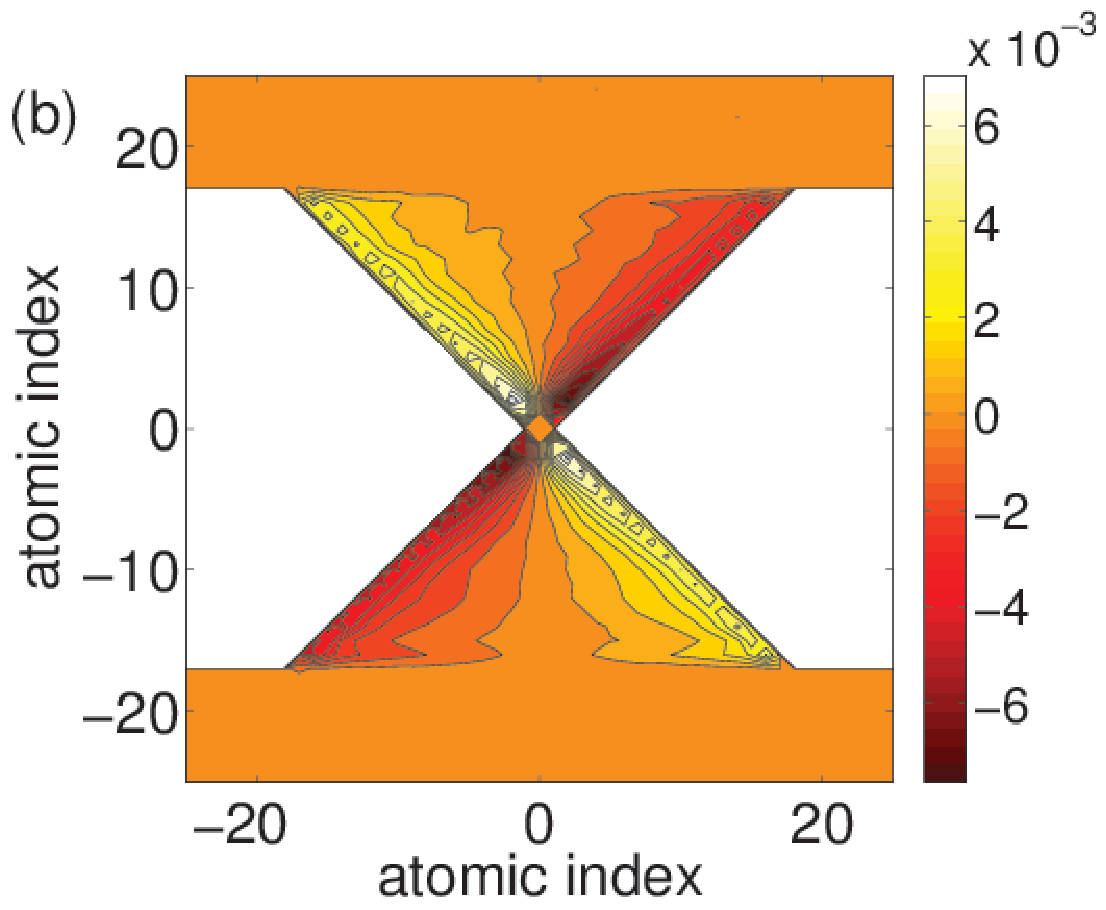
\includegraphics[width=.49\columnwidth]{pics/aip_fig5b.pdf}
 \caption{Kinetic temperature profile in (a) triangular and (b) discoidal constriction at low temperature. Figure reprinted with publisher's permission from \citepub{fpu2}. \textbf{FIX ANNOTATION IN B}}
\label{fig:aip_figs56}
\end{center}
\end{figure}

To investigate the effects of the constriction geometry on interference effects at low temperatures, calculations were performed also for hour-glass shaped and discoidal constrictions. Kinetic temperature profiles for these geometries are shown in Fig. \ref{fig:aip_figs56}. For the small contact areas shown here, temperature profiles in the bulk parts are essentially constant due to the small thermal contact between the upper and lower parts of the structure. In the triangular point contact, temperature changes nearly linearly as the constriction becomes narrower. Spatial analysis of the local heat current presented in \citepub{fpu2} reveals that heat flows mainly along the edges of the triangles. In the discoidal geometry of Fig. \ref{fig:aip_figs56}(b), which could represent a nanoparticle sandwiched between two materials, temperature profile is again nearly flat inside the center region, with only small spatial variations in temperature. However, local heat currents inside the center region, shown in \citepub{fpu2}, are strongly direction-dependent, with similar enhancement in $\langle 11\rangle$ direction as in the temperature profile of Fig. \ref{fig:fpu_fig2}(a).

The results show that in the ballistic low-temperature limit, local temperature and heat current profiles can exhibit wavelike-features with interference patterns. Accounting for such directional patterns could enable more efficient engineering of thermal conductivity in nanostructures. It is, however, well known that quantum statistics neglected by classical molecular dynamics is most significant at low temperatures. To include quantum statistics, we turn to the quantum-mechanical Green's function method based on the linearized Langevin equations of motion presented in Sec. \ref{sec:th_eom}.

\section{Langevin modeling of phononic and photonic energy transfer}
\label{sec:results_gf}

As discussed in Sec. \ref{sec:th_eom}, solving the linearized Langevin equations \eqref{eq:th_eom1}, \eqref{eq:th_eom2}, and \eqref{eq:th_eom3} in terms of the Green's function allows for heat transfer modeling that accounts for wave interference, quantum statistics, and even dissipative losses in terms of a frequency-independent relaxation rate. In this thesis, Green's function method is applied to investigate (i) quantum thermal transport through point contacts in Subsection \ref{sec:results_schb} and (ii) cavity-enhancement of electromagnetic energy transfer rates between SiC nanoparticles in Subsection \ref{sec:results_cavity}. % These analysis are based on solving the linearized Langevin equations of motion for phonons and photons, respectively, presented in Sec. \ref{sec:th_eom}. Quantum effects are incorporated through the quantum-mechanical fluctuation-dissipation theorem for Langevin noise terms (Sec. \ref{sec:th_langevin}) and dissipation effects through the Langevin damping terms accompanying the noise terms. % Losses are incorporated in the models through the Langevin terms. %Section \ref{sec:results_schb} presents quantum temperature profiles for rectangular point contacts ontacts and Section \ref{sec:results_cavity}  and (ii) electromagnetic energy transfer between nanoparticles in a mirror cavity. These results were published in Publications \cp{gf} and \cp{dipole}, respectively. 

\subsection{Quantum effects in point contacts}
\label{sec:results_schb}

Application of the linearized Langevin equation \eqref{eq:th_eom1} for lossy phonon transport is closely related to the self-consistent heat bath model \cite{bolsterli70}, discussed in more detail below. Whereas earlier works have applied the model to simple one-dimensional systems (see, e.g., Refs. \cite{bolsterli70,visscher75,dhar03,dhar06,segal09,bandyopadhyay11}) with a finite number of atoms, \citepub{gf} extended the model to more complex geometries with an infinite number of atoms.  %The model was then applied to investigating quantum temperature profiles in constrictions in rectangular lattices and graphene.

The setup of \citepub{gf} is schematically illustrated in Fig. \ref{fig:schb_setup}. The setup consists of a center region with a finite number of atoms and left and right leads with possibly an infinite number of atoms. All atoms are coupled to local Langevin baths mimicking all interaction events driving the system towards local thermal equilibrium \cite{bolsterli70}. In the center region of Fig. \ref{fig:schb_setup}(a), a point contact acts as a scattering center for phonons coming in from the left and right leads. In the vicinity of the contact, bath temperatures are unknown. Following the self-consistent heat bath model \cite{bolsterli70}, they are determined self-consistently from the requirement that the heat current to each bath vanishes. The requirement of zero heat current to local baths ensures that the heat current flowing in the chain is conserved at each atom site, a natural requirement in the steady-state in the absence of electron-phonon or electron-photon coupling.

Away from the scattering region, the baths are set to prescribed temperatures $T_L$ and $T_R$. Whereas earlier works \cite{dhar06} have modeled lattice dynamics in the leads as completely lossless, which induces an acoustic mismatch between the lossless leads and the lossy center region, the setup of Fig. \ref{fig:schb_setup} eliminates this mismatch by including losses for the leads as well.  % The baths then  act as quantum-mechanical temperature probes. 


\begin{figure}
\begin{center}
 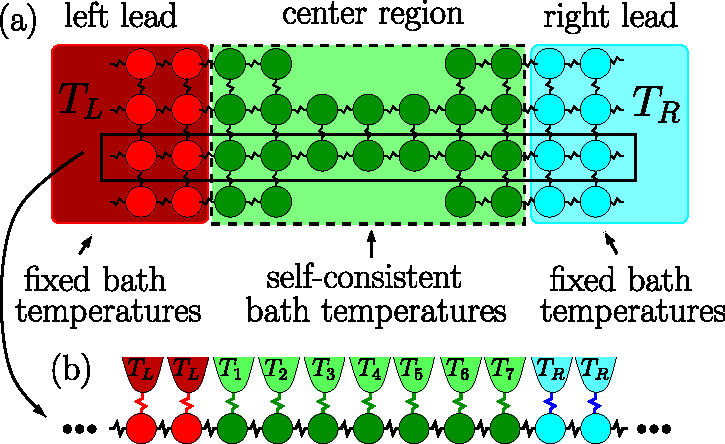
\includegraphics[width=.99\columnwidth]{pics/gf_fig1.pdf}
 \caption{A schematic illustration of the self-consistent heat bath model for a constriction in a two-dimensional rectangular lattice. The system consists of the left lead, the center region, and the right lead. All atoms are coupled to Langevin heat baths, shown explicitly for one cross section in (b). Whereas the temperatures of the Langevin baths have prescribed values $T_L$ and $T_R$ in the left and right lead, the bath temperatures are determined self-consistently in the center region from the requirement that the thermal current to each bath is zero \cite{bolsterli70}. Reprinted from \citepub{gf} with publisher's permission.}
\label{fig:schb_setup}
\end{center}
\end{figure} 

The calculation of heat currents starts from the Langevin equation of motion \eqref{eq:th_eom1} for each atom $i$ with interatomic force constants $\bb{K}_{ij}$ determined by the interatomic potential energy function. The relaxation rate $\gamma$ is chosen to correspond to known phonon life-times. It is shown in \citepub{gf} that solving the equations of motion for the leads and substituting to the equations for the center region allows for replacing the leads by \textit{single} Langevin heat baths at temperatures $T_L$ and $T_R$, which reduces the number of degrees of freedom to those in the center region. The microscopic details of acoustically matched lattice dynamics in the leads are fully captured by the lead self-energy functions $\Sigma^L(\omega)$ and $\Sigma^R(\omega)$. Microscopic definitions of the self-energy function in terms of the lead Green's function and the fluctuation-dissipation theorem for the corresponding Langevin noises are presented in detail in \citepub{gf}.



% The self-consistent bath model can be similarly extended for complex electron systems to study local heating and thermoelectric effects in quantum transport \cite{roy07}. 
% The heat current to each local bath at site $i$ can be determined by calculating the rate of change of local energy \cite{hardy63}, which reads in the harmonic approximation
% \begin{equation}
%  e_i = \frac{1}{2}m\dot{\bu}_i^2 + \frac{1}{2} \sum_{\alpha,\beta}\sum_j u_i^{\alpha} K_{ij}^{\alpha\beta} u_j^{\beta} . \label{eq:th_ei}
% \end{equation}
% Calculating the time derivative of Eq. \eqref{eq:th_ei} and thermal averaging gives
% \begin{equation}
%  \langle \dot{e}_i \rangle = -\sum_j  J_{ij} -  Q_i ,
% \end{equation}
% where the first term in brackets on the right hand side corresponds to the heat current
% \begin{equation}
%  J_{ij} = \frac{1}{2} \sum_{\alpha,\beta} \left\langle \dot{u}_i^{\alpha}K_{ij}^{\alpha\beta} u_j^{\beta} - u_i^{\alpha} K_{ij}^{\alpha\beta} \dot{u}_j^{\beta} \right\rangle
% \end{equation}
% between particles $i$ and $j$ and the second term is the heat flow to the bath, defined as 
% \begin{equation}
%  Q_i = \langle [m\gamma \dot{\bu}_i-\xi_i] \cdot \bu_i \rangle.
% \end{equation}


By following the procedure presented in Sec. \ref{sec:th_bathcurrents}, one can calculate the heat currents flowing to baths in terms of the center region's Green's function $\bb{G}(\omega)$. By setting the heat current equal to zero for the local baths in the center region, one gets a non-linear system of equations for the bath temperatures. This system of equations can be solved by, e.g., using Newton-Raphson method \cite{bandyopadhyay11} or resorting to linearizing approximations \cite{segal09}. It is shown in \citepub{gf} that the requirement of vanishing heat current to the baths is equivalent to an intuitive thermal balance condition between kinetic and potential energies. Similar thermal balance condition was recently reported for local photon number in fluctuational electrodynamics \cite{partanen14}. % The self-consistent temperature profile and the evaluation of heat currents flowing to the two leads then constitute a solution of the vibrational heat transfer problem. %  temperature ensures local energy balance between the kinetic and potential energies. % Results for constrictions in two-dimensional lattices are presented in Sec. \ref{sec:results_gf}. %The transmission function is given by Eq. \eqref{eq:th_caroli} and $\Gamma^I(\omega)=-2\textrm{Im}[\Sigma^I(\omega)]$ is the bath coupling function, as again explained in \citepub{gf}.



% 

%The similarities of the equations of motion become more apparent in the linear approximation, which is discussed in more detail below. In this case, the force acting on atom $i$ becomes $F_i^{\alpha}=-\sum_{j}\sum_{\beta} K_{ij}^{\alpha\beta}u_j^{\beta}$ and the electron Hamiltonian 

% \subsubsection{Electromagnetic energy transfer in a cavity}

\begin{figure}
 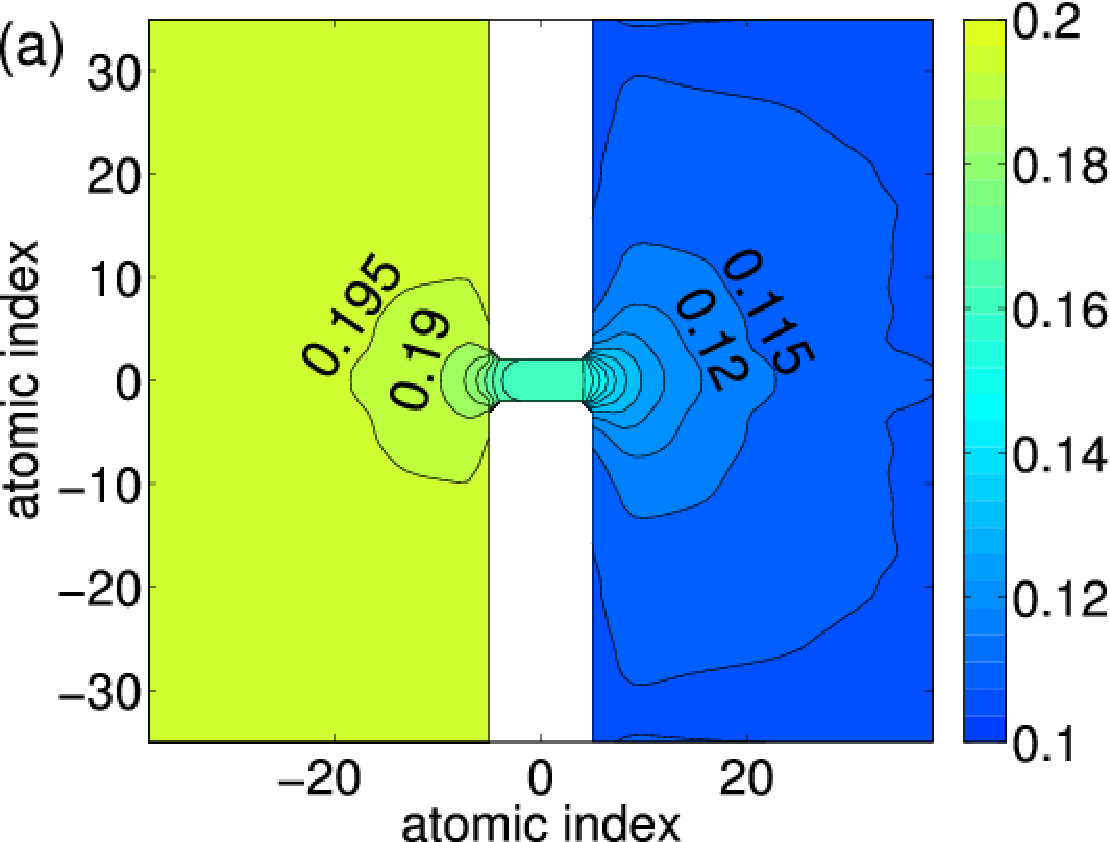
\includegraphics[width=.49\columnwidth]{pics/gf_fig7a.pdf}
 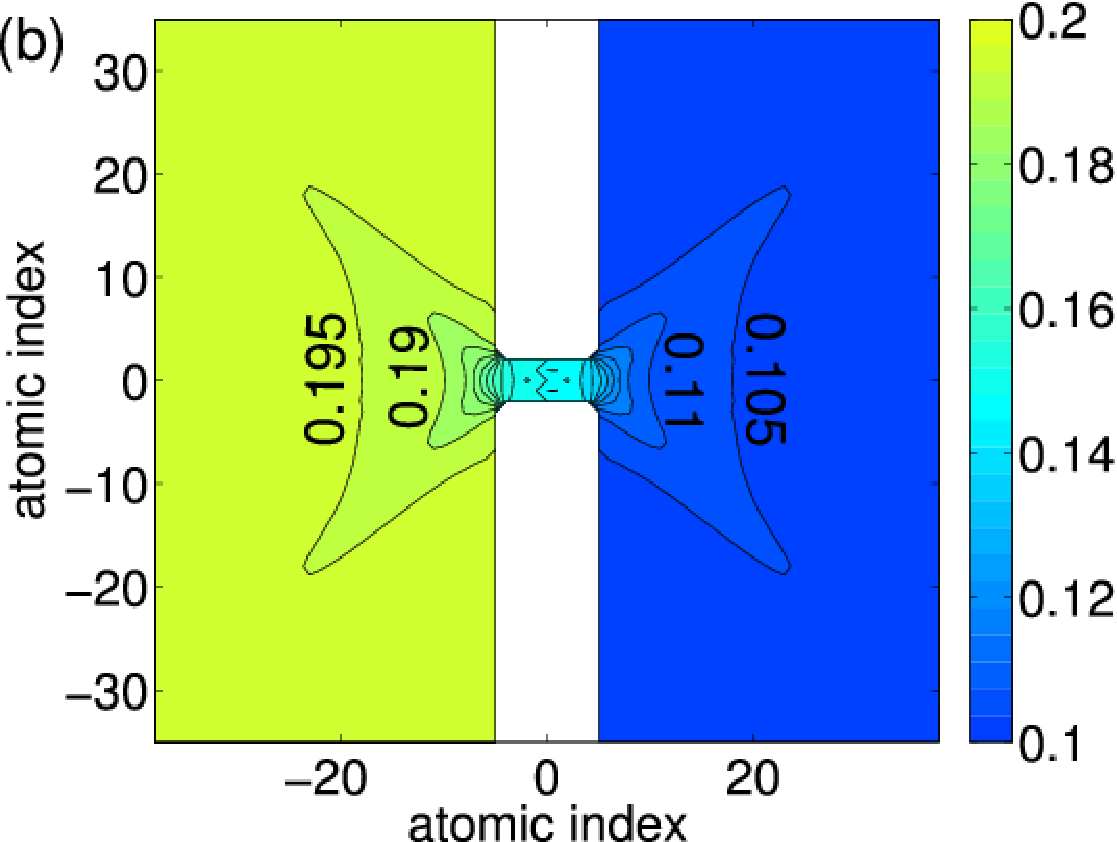
\includegraphics[width=.49\columnwidth]{pics/gf_fig7b.pdf}
 \caption{Self-consistent local bath temperature profiles in a rectangular constriction. Lead temperatures are $T_L=0.2$ and $T_R=0.1$. Figures show temperature profiles for (a) quantum and (b) classical statistics. Friction parameter is $\gamma=0.01$, corresponding to nearly ballistic transport. Figure reprinted with publisher's permission from \citepub{gf}.}
 \label{fig:gf_fig7}
\end{figure}

As an application of the formalism, we investigated quantum effects in thermal transport through a rectangular point contact in a square lattice, considered in Sec. \ref{sec:results_interference} by classical molecular dynamics. Nearest neighbors were connected by harmonic springs and weak dissipative losses were included through the bath dissipation parameter $\gamma=0.01$ in the units of spring resonance frequency (see \citepub{gf}). Figure \ref{fig:gf_fig7} shows temperature profiles for (a) quantum and (b) classical statistics. In this case, the directional features observed in the classical case of Fig. \ref{fig:gf_fig7}(b) and molecular dynamics results of Fig. \ref{fig:fpu_fig2}(a) are washed away by quantum statistics. This suggests that the directional features observed in the classical case arise from high-frequency modes, whose population is overestimated by classical statistics.

To see if interference effects could be observed in a more realistic system, we studied quantum thermal transport through a graphene point contact depicted in Fig. \ref{fig:gf_fig8}(a). Determining temperature profiles for such a system from classical methods such as molecular dynamics simulation might be very inaccurate due to the high Debye temperature of graphene, requiring turning to quantum-mechanical Green's function calculations. The drawback is that anharmonic phonon scattering is only included in terms of a single relaxation time $\gamma^{-1}=1$ ps, which we take to correspond to the experimentally measured phonon life-time \cite{bonini12}. The interatomic force constants $\bb{K}_{ij}$ are taken from the fourth-nearest-neighbor force constant model \cite{saito} with the parameters of Ref. \cite{wirtz04}. %The bath relaxation time $\gamma$ is chosen to correspond to the acoustic phonon life-time $\gamma^{-1}=1$ ps, which is the approximate value measured experimentally \cite{bonini12}.

\begin{figure}
 \begin{center}
 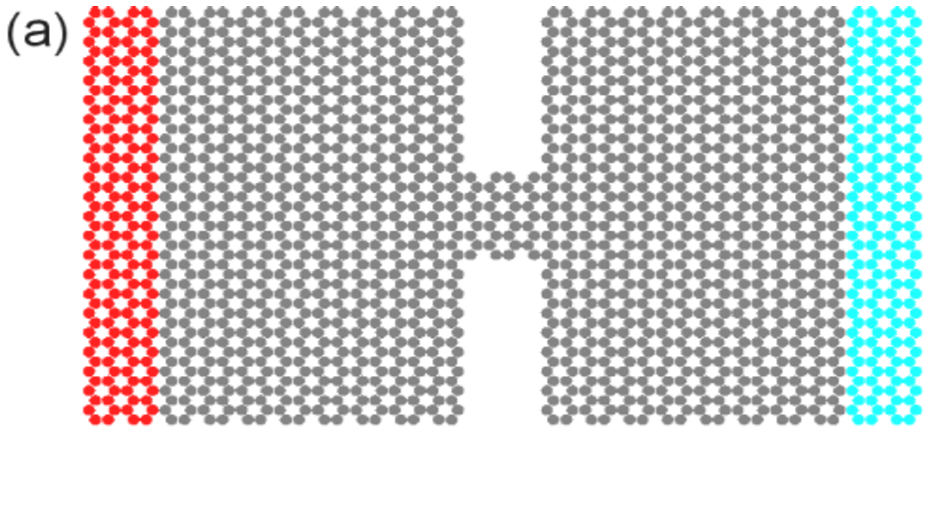
\includegraphics[width=.49\columnwidth]{pics/gf_fig8a.pdf}
 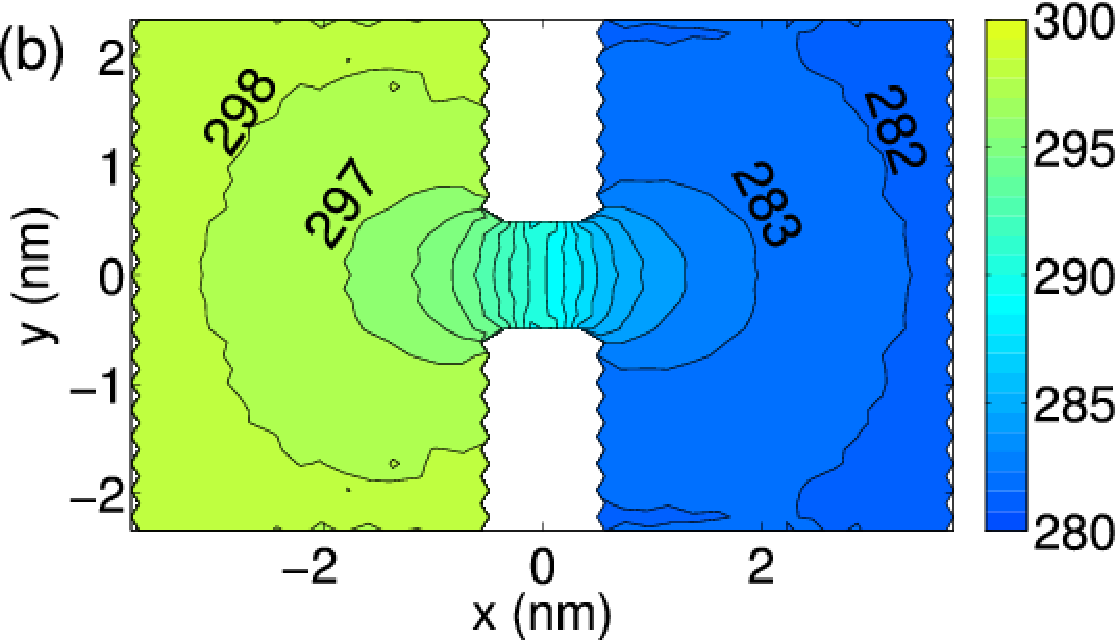
\includegraphics[width=.49\columnwidth]{pics/gf_fig8b.pdf}
 \end{center}
 \caption{(a) Illustration of a point contact in graphene. The leads (red and cyan atoms) extend infinitely to the left and right, but the temperatures are determined self-consistently only for the center region (gray atoms). (b) Self-consistent bath temperature profiles (K). The semi-infinite leads are at temperatures $T_L=300$ K and $T_R=280$ K. Phonon relaxation time $\tau=1/\gamma$ is set to $1$ ps. Figure reprinted with publisher's permission from \citepub{gf}.}
 \label{fig:gf_fig8}
\end{figure}

The calculated temperature profile in the graphene point contact is plotted in Fig. \ref{fig:gf_fig8}(b) for lead temperatures $T_L=300$ K and $T_R=280$ K. In the considered geometry, there are no visible interference effects in temperature profiles. Quantum effects are observable in the slight asymmetry in temperature profiles at different sides of the junction: purely classical statistics would produce a fully symmetric temperature profile due to the linearity of the self-consistent equations for bath temperatures, as discussed in \citepub{gf}.

The same principles as outlined here for phonon transport can be directly applied to electron transport as well, when the equations of motion for lattice vibrations (Eq. \eqref{eq:th_eom1}) are replaced by the electronic ones (Eq. \eqref{eq:th_eom3}). In electron transport, the self-consistent baths are often referred to as voltage-temperature probes \cite{jacquet09}. Applications of voltage-temperature probe models for describing dissipation effects in electron transport have been so far limited only to one-dimensional geometries \cite{buttiker86,damato90,jacquet09,jacquet12}, although the model can account for wave dynamics, Joule heating as well as thermoelectric effects \cite{roy07} in complicated geometries. Recently, Bergfield \textit{et al.} used the model for investigating quantum temperature oscillations in electrically biased graphene \cite{bergfield15}.

\subsection{Cavity-modified electromagnetic energy transfer (\citepub{dipole})}
\label{sec:results_cavity}

\begin{figure}
 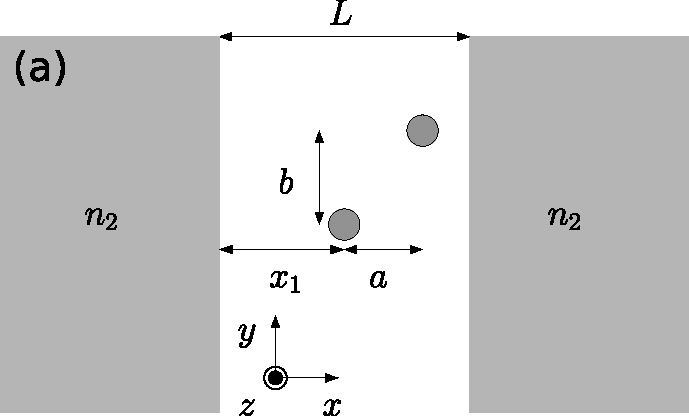
\includegraphics[width=.55\columnwidth]{pics/dipole_fig2.pdf}
 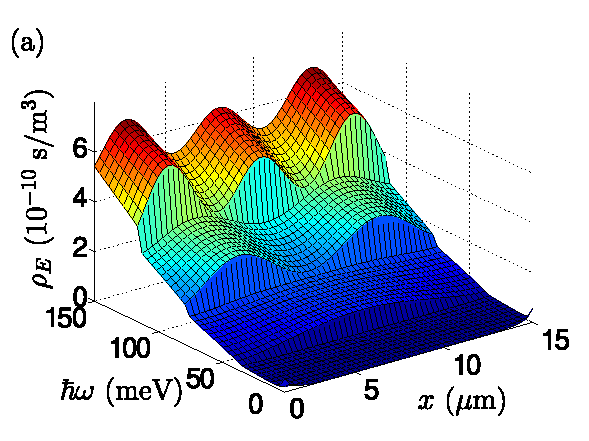
\includegraphics[width=.44\columnwidth]{pics/dipole_fig3a.pdf}
 \caption{(a) Schematic illustration of two nanoparticles located in a mirror cavity of length $L$. One of the particles is located at the middle of the cavity and the position of the second particle is defined by parameters $a$ and $b$ as shown in the figure. The refractive index of the cavity walls is denoted by $n_2$. (b) Electromagnetic density of states as a function of position and energy for a cavity with $L=16$ $\upmu$m and $n_2=2+20i$. The lowest-frequency standing waves have cut-off energies 37.6 meV, 76.3 meV, and 115.1 meV. These modes can couple to the absorption resonance of SiC nanoparticles at $\hbar\omega_r=115.6$ meV. Figure reprinted with publisher's permission from \citepub{dipole}. \textbf{FIX A AND B}}
\label{fig:gfm_dipole_system}
\end{figure}

% We briefly outline the quantum Langevin equation approach to the electromagnetic energy transfer here. The final results for energy transfer rates are equivalent to those calculated from fluctuational electrodynamics \cite{benabdallah11,messina13}, as explained in \citepub{dipole}. 

In 1946, Purcell \cite{purcell46} suggested that spontaneous emission from an oscillating dipole could be enhanced by placing the oscillator in a resonant cavity, effectively increasing the electromagnetic density of states. The possibility to tune the rate of spontaneous emission has since been demonstrated also experimentally (see, e.g., Ref. \cite{hulet85} and references therein), and such tuning is now routinely applied in, e.g., optoelectronics \cite{} and optomechanics \cite{}.

Purcell effect raises the natural question of whether it is possible to similarly tune the thermal conductance between electromagnetically coupled dielectric bodies. Unlike near-field enhancement of energy transfer, such cavity-tuning is expected to persist at large distances and could be applied, e.g., for (i) enhancing thermal coupling between dielectric bodies, allowing for efficient cooling of hot spots, or (ii) suppressing thermal coupling, preventing undesired propagation of heating. 


%  As discussed in Chap. \ref{chap:intro}, it is well known that thermal conductance strongly increases in the near-field, but such near-field enhancement is always limited to distances at the order of thermal wavelength.

% We apply the quantum Langevin equations to investigate the cavity-enhancement of electromagnetic energy transfer rates between two spherical SiC nanoparticles at different temperatures. These results are published in \citepub{dipole}. 

The system studied in \citepub{dipole} is schematically depicted in Fig. \ref{fig:gfm_dipole_system}(a). Two SiC nanoparticles are located in a microcavity formed by two half-spaces with refractive index $n_2=2+20i$ and separated by distance $L$. Due to cavity confinement, the electromagnetic field forms standing waves in the cavity, which can be seen as ''stairs'' in the electromagnetic density of states shown in Fig. \ref{fig:gfm_dipole_system}(b). For $L=16$ $\upmu$m, the lowest-energy standing waves can be excited at 37.6 meV, 76.3 meV, and 115.1 meV. The length of the cavity $L=16$ $\upmu$m is chosen such that only these three low-energy modes can couple electromagnetically to the SiC nanoparticle resonance at 115.6 meV (see below). % Due to the confinement of electromagnetic modes in the mirror cavity, the coupling of the electromagnetic field to the nanoparticles depends on the position and 

The radius of the nanoparticles is assumed to be $R=250$ nm and the relative dielectric constant $\varepsilon(\omega)$ of SiC is modeled by the Lorentz model \cite{mulet01,spitzer59}. The Clausius-Mossotti polarizabilities of the particles are given by
\begin{equation}
 \alpha^{\textrm{CM}}(\omega)= 4 \pi R^3 \frac{\varepsilon(\omega)-1}{\varepsilon(\omega)+2} \unitdyadic.
\end{equation}
The particles have strong absorption peaks at the phonon-polariton resonance energy $\hbar \omega_r=115.6$ meV corresponding to $\textrm{Re}[\varepsilon(\omega)]=-2$, which forces the interparticle energy transfer to be nearly monochromatic. As discussed above, only three lowest-energy standing waves can be excited in the $L=16$ $\upmu$m cavity at this frequency, and the coupling of the particles to the electromagnetic field therefore depends strongly on the positions of the particles.  % The dependence of particle distances $a$ and $b$ on electromagnetic energy transfer rates is investigated below. %  Consequently, thermal energy transfer between the nanoparticles is nearly monochromatic and one can tune the interparticle energy transfer by tuning the cavity resonances. By choosing the cavity length $L=16$ $\mu$m, the lowest cavity resonances are located at  Only these modes can 

\begin{figure}
 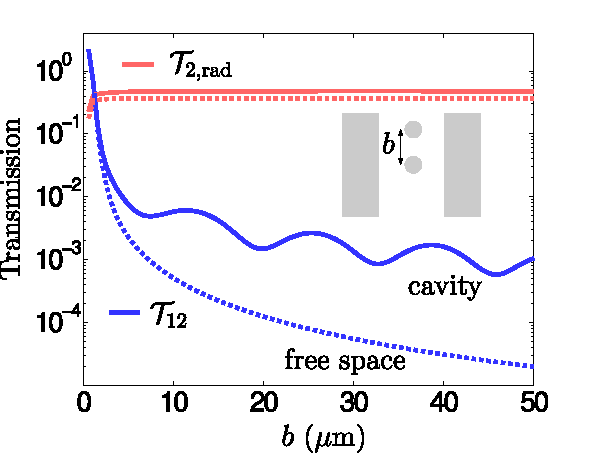
\includegraphics[width=.79\columnwidth]{pics/dipole_fig5.pdf}
 \caption{Energy transmission function $\ca{T}_{12}(\omega_r)$ between two SiC nanoparticles at the nanoparticle resonance frequency $\omega_r$ as a function of vertical separation $b$ (see the inset). The mirror cavity enhances the interparticle thermal conductance and gives rise to interference effects seen as conductance oscillations as a function of distance. The cavity also enhances the coupling between the environment and each dipole, as indicated by the larger dipole-environment transmission function $\ca{T}_{2,\textrm{rad}}(\omega_r)$ with mirror cavity (solid red line) than in free-space (dashed red line). Figure reprinted with publisher's permission from \citepub{dipole}.}
\label{fig:dipole_fig5}
\end{figure}

Figure \ref{fig:dipole_fig5} shows the dipole-dipole transmission $\ca{T}_{12}(\omega_r)$ and the dipole-environment transmission $\ca{T}_{2,\textrm{rad}}(\omega_r)$ at the resonance energy $\hbar\omega_r=115.6$ meV as a function of the vertical distance $b$. The interparticle transmission $\ca{T}_{12}(\omega_r)$ in the cavity (solid blue line) can be seen to exceed the free-space value (dashed blue line) at distances larger than $b\approx 2$ $\upmu$m. In addition, the transmission oscillates as a function of distance due to the interference between electromagnetic cavity modes. As shown in \citepub{dipole}, interparticle thermal conductance can be similarly enhanced also by placing the particles close to a SiC surface supporting surface phonon polaritons.

These results suggest that electromagnetic energy transfer rates between particles can be tuned by modifying the electromagnetic environment, in analogy with the Purcell tuning of radiative emission. Increasing the coupling to the electromagnetic field increases, however, also the thermal coupling to the environment, which may overshadow the interparticle energy transfer. Heat flow from the particles to the environment could be reduced by, e.g., cooling the cavity walls. 

